\documentclass[11pt]{amsart}
\usepackage[margin=1.15in]{geometry}
\usepackage{amssymb,amsmath,mathtools}
\usepackage{graphicx,booktabs,array,float}
\usepackage[section]{placeins}
\usepackage[hidelinks]{hyperref}
\usepackage[expansion=false]{microtype}

\newtheorem{theorem}{Theorem}[section]
\newtheorem{proposition}[theorem]{Proposition}
\newtheorem{lemma}[theorem]{Lemma}
\newtheorem{corollary}[theorem]{Corollary}
\newtheorem{mainthm}{Theorem}
\renewcommand{\themainthm}{\Alph{mainthm}}
\theoremstyle{definition}
\newtheorem{definition}[theorem]{Definition}
\newtheorem{remark}[theorem]{Remark}
\newtheorem{example}[theorem]{Example}
\newtheorem{conjecture}[theorem]{Conjecture}

\newcommand{\ZZ}{\mathbb{Z}}
\newcommand{\QQ}{\mathbb{Q}}
\newcommand{\CC}{\mathbb{C}}
\newcommand{\Tr}{\operatorname{Tr}}
\newcommand{\Crit}{\operatorname{Crit}}
\newcommand{\cM}{\mathcal M}
\newcommand{\cR}{\mathcal R}
\newcommand{\cW}{\mathcal W}
\newcommand{\GL}{\mathrm{GL}}
\newcommand{\PG}{\mathrm{P}G}
\newcommand{\NTHREEUPPER}{[UPPER]}
\newcommand{\zenodoDOI}{10.5281/zenodo.XXXXXXXX}

\setlength{\emergencystretch}{2.5em}
\hbadness=2000
\raggedbottom
\begin{document}

\title[Zero angular momentum of D-brane microstates]{Black Hole Microstates of Two and Three\\ D6-Branes Carry No Angular Momentum}

\author{Deep Bhattacharjee}
\address{Formerly, Electro-Gravitational Space Propulsion Laboratory (EGSPL), Bhubaneswar, Odisha 751030, India}
\address{Formerly, University of Calcutta (Heramba Chandra College), 23/49 Gariahat Road, Golpark, Kolkata 700029, West Bengal, India}
\email{d.bhattacharjee@erl-forschung.de}
\email{itsdeep@live.com}
\email{egspl@proton.me (GitHub-related contact; GitHub account creelie)}
\urladdr{https://orcid.org/0000-0003-0466-750X}

\begin{abstract}
For the D2-D2-D2-D6 system on $T^6$ with any number of D6-branes, every classical supersymmetric vacuum is a simple quiver representation; the vacua are therefore the critical points of one function on a smooth space, and they come in pairs. With one D6-brane they are exactly $12$ isolated points for generic moduli, and with two and three D6-branes exactly $56$ and $208$ isolated points at explicit moduli, as Sen's zero angular momentum conjecture predicts.
\end{abstract}

\maketitle

\noindent\textbf{Keywords:} black hole microstates; quiver quantum mechanics; zero angular momentum.

\smallskip\noindent\textbf{MSC 2020:} 81T60 (primary); 16G20, 14L24, 13P10, 83E30.

\section{Introduction}\label{sec:intro}

A supersymmetric black hole in four dimensions has a spherically symmetric horizon. Sen observed that the near-horizon geometry $AdS_2\times S^2$ then forces every microstate of a single-centred black hole, once the fermion zero modes of the broken supersymmetries are removed, to be a singlet of the rotation group $SU(2)$ \cite{Sen11,DGMS11}.\footnote{The argument is that the near-horizon $SU(1,1|2)$ symmetry contains the rotation group, and that the black hole entropy counts states in the $AdS_2$ ground state, which is annihilated by all the generators of $SU(1,1|2)$, including $\vec J$. The relation between the index and the degeneracy that follows from it is derived in \cite{DGMS11}.} In particular the protected index of such a black hole equals its degeneracy and is positive. The statement is about the black hole, where the string coupling is large. Chowdhury, Garavuso, Mondal and Sen proposed a stronger form: at a generic point of the moduli space of the compactification, even in the weakly coupled region where the microstates are described by D-branes, all the microstates of a single-centred black hole carry zero angular momentum \cite{CGMS14,CGMS16}.

The strong form can be tested in type~II string theory on $T^6$. There, for the charges carried by black holes, multi-centred configurations do not contribute to the index \cite{Sen08b}, and the index itself is known exactly from the $\mathcal N=8$ counting formula \cite{SSY06,Sen10}. Chowdhury, Garavuso, Mondal and Sen studied $N_1$, $N_2$, $N_3$ D2-branes wrapped on the three two-tori $T^2_{45}$, $T^2_{67}$, $T^2_{89}$ of $T^6=T^2_{45}\times T^2_{67}\times T^2_{89}$ together with $N$ D6-branes wrapped on all of $T^6$. With $N_1=N_2=N_3=1$ the low energy dynamics is a quantum mechanics with gauge group $U(1)^3\times U(N)$ and four supercharges, the dimensional reduction of an $\mathcal N=1$ gauge theory in four dimensions (Figure~\ref{fig:quiver}). The BPS states are the harmonic forms on the space $\cM$ of classical vacua, with the rotation group acting as the Lefschetz $SU(2)$ \cite{Wit82,Den02,BBdBES12}. The strong conjecture therefore says that $\cM$ is a finite set of points, and its number of points must be the index
\begin{equation}\label{eq:prediction}
-\hat c(4N)=12,\ 56,\ 208,\ 684,\ 2032,\ 5616,\ldots\qquad(N=1,2,3,4,5,6,\ldots),
\end{equation}
where $\hat c(4N)$ is the coefficient of $q^Ny^0$ in $-\vartheta_1(z|\tau)^2/\eta(\tau)^6$ (Appendix~\ref{app:prediction}).

In \cite{CGMS14} the vacua were found for $N=1$, and in \cite{CGMS16} for $N=2$ and $N=3$: $12$, $56$ and $208$ isolated solutions of the $F$-term equations in a fixed gauge, at random rational values of the parameters, with Hilbert series computed in Singular and Macaulay2 and numerical solutions as a check; configurations where the gauge choice fails were examined separately and gave no solutions. For $N=2$ the $D$-term equations and the gauge field potential were then analysed solution by solution. For $N=3$ the authors state that they did not check explicitly that each solution of the $F$-term equations carries a unique solution of the $D$-term equations, and expected it on general grounds \cite[Section~5]{CGMS16}. No case beyond $N=3$ has been computed.

In this paper we settle the structure for every $N$ and the counts for $N\le 3$. Let $\cM_c$ be the space of vacua, at values $c$ of the parameters of the superpotential, modulo gauge transformations and modulo the flat directions of the centre of mass. Write $\cR^{\rm s}$ for the space of simple representations of the quiver, $\PG$ for the gauge group modulo its centre and $f_c$ for the function induced by the superpotential on the smooth variety $\cR^{\rm s}/\PG$.

\begin{mainthm}\label{thm:A}
Let $N\ge1$ and let the parameters $c^{(k\ell)}$ of the superpotential be nonzero. Every solution of the $F$-term equations is a simple representation of the quiver. Consequently, for every value of the Fayet--Iliopoulos parameters:
\begin{enumerate}
\item every complex gauge orbit of $F$-term solutions contains exactly one unitary orbit of solutions of the $D$-term equations;
\item at every vacuum the gauge fields vanish up to the overall translation, so the gauge field potential imposes nothing further;
\item $\cM_c$ is the critical locus of $f_c$ on the smooth variety $\cR^{\rm s}/\PG$, taken modulo the shift symmetries;
\item the map $x\mapsto -x$ on all chiral fields induces an involution of $\cM_c$ without fixed points. In particular, whenever $\cM_c$ is finite, its number of points is even.
\end{enumerate}
\end{mainthm}

Part~(iv) explains why every number in \eqref{eq:prediction} is even. Part~(iii) turns the conjecture into a question about the critical points of one function on a smooth space, and we use it to give exact counts.

\begin{mainthm}\label{thm:B}
\begin{enumerate}
\item For $N=1$ and all values of $c$ outside a proper Zariski-closed subset, $\cM_c$ consists of exactly $12$ points.
\item For $N=2$ and $N=3$ there are explicit rational parameters $c_0$ (Table~\ref{tab:c0}) at which $\cM_{c_0}$ consists of exactly $56$, respectively $208$, points, each a nondegenerate critical point of $f_{c_0}$. The count is exact: no vacuum is lost to the choice of gauge.
\item For $N=2,3$ and every $c$ close to $c_0$, $\cM_c$ contains at least $56$, respectively $208$, nondegenerate vacua, and the same lower bound holds for all $c$ outside a proper Zariski-closed subset.
\end{enumerate}
\end{mainthm}

In each case the vacua are isolated, so $P(y)$ is a constant and all BPS states have $J_3=0$: the strong zero angular momentum conjecture holds at these parameters, with the counts \eqref{eq:prediction}. Theorem~\ref{thm:A}(i) supplies the step that was left open for $N=3$ in \cite{CGMS16}, and does so for every $N$. The statement for $N=2,3$ at $c_0$ is a theorem: the number of solutions of the gauge-fixed equations is computed with exact rational arithmetic, it is matched by an explicit list of algebraic solutions, each of which is checked to satisfy every equation identically, and the configurations excluded by the gauge choice are shown to contain no solution.\footnote{All computations are exact over $\QQ$; no floating point number enters a proof. The programs are archived at \cite{Bha26}.} For $N=4$ we find exactly $684=-\hat c(16)$ vacua in a gauge slice modulo a large prime (Section~\ref{ssec:N4}); this is not a proof.

\begin{figure}[t]
\centering
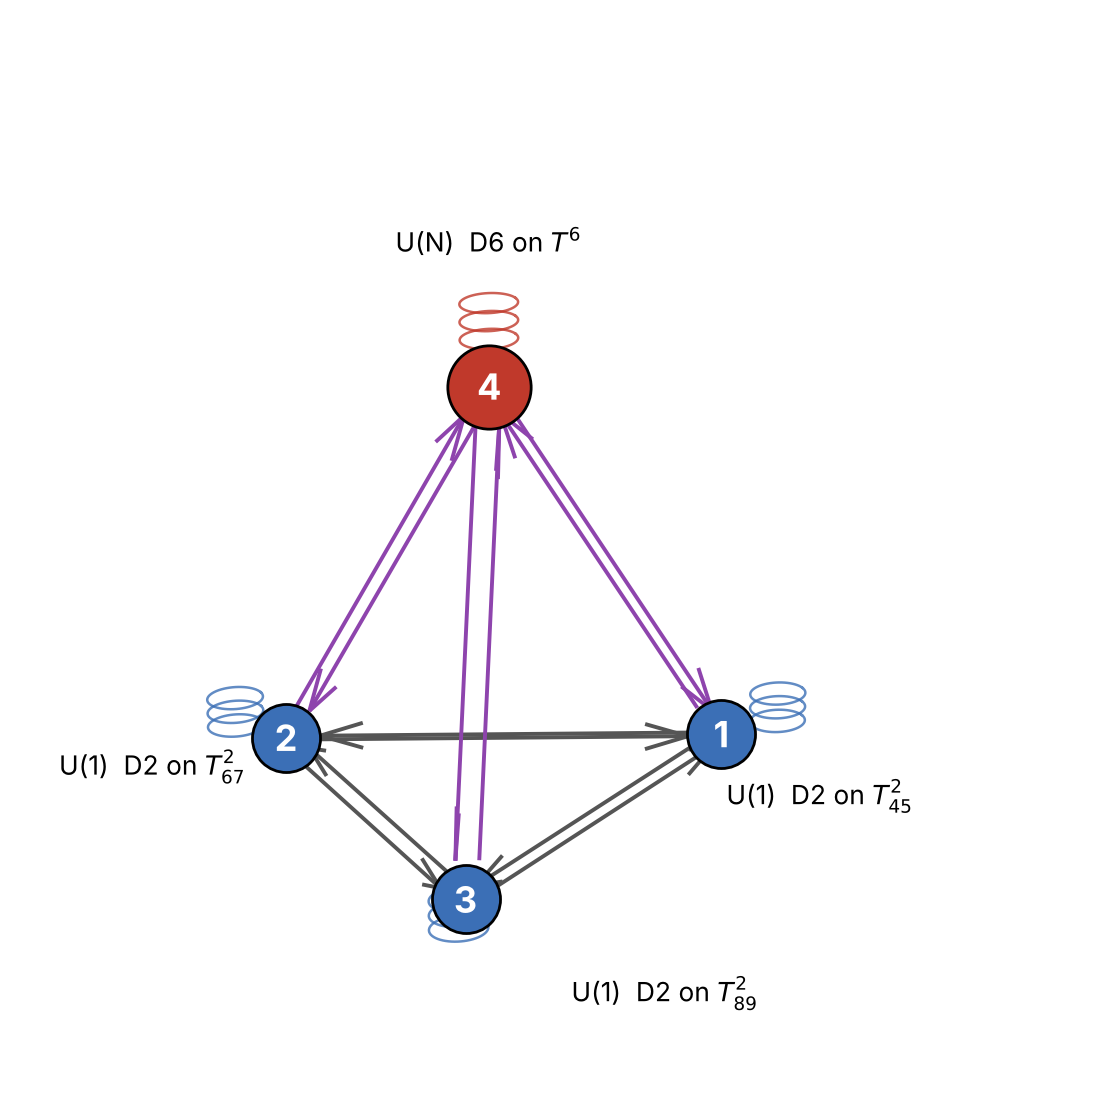
\includegraphics[width=0.62\textwidth]{figures/fig_quiver.png}
\caption{The quiver of the D2-D2-D2-D6 system drawn on a tetrahedron. Nodes $1,2,3$ carry $U(1)$ and node $4$ carries $U(N)$. Each edge carries the two bifundamental fields $Z^{(k\ell)}$ and $Z^{(\ell k)}$, and each node carries three adjoint fields $\Phi^{(k)}_1,\Phi^{(k)}_2,\Phi^{(k)}_3$, drawn as loops.}
\label{fig:quiver}
\end{figure}

The proof of Theorem~\ref{thm:A} is short. The $F$-term equations for the adjoint fields say that the products of the bifundamentals around each edge are nonzero constants, and that on the $U(N)$ node the commutators of the adjoints are $-c^{(k4)}$ times the identity modulo a rank one matrix. A proper subrepresentation would make the commutator equation hold on a nonzero quotient or subspace with the rank one term removed, and taking the trace there gives $-c^{(k4)}$ times its dimension equal to zero. Simplicity then gives the $D$-terms by King's theorem \cite{Kin94}, the gauge fields by Schur's lemma, and the pairing by the oddness of the superpotential.

Theorem~\ref{thm:B} rests on a gauge slice that is valid at every simple representation where certain rows are independent, on exact elimination for the slice equations, and on separate exact computations showing that the configurations where these rows are dependent carry no vacua. The rational univariate representation of the solutions \cite{Rou99} gives a certificate that can be checked independently of the program that produced it.

The paper is organised as follows. Section~\ref{sec:system} recalls the quantum mechanics and states the conjecture precisely. Section~\ref{sec:simple} proves Theorem~\ref{thm:A}. Section~\ref{sec:slices} constructs the gauge slices and proves that they miss no vacuum. Section~\ref{sec:counts} proves Theorem~\ref{thm:B}. Section~\ref{sec:discussion} discusses what remains open. Appendix~\ref{app:fterms} lists all $F$-term equations, Appendix~\ref{app:prediction} derives \eqref{eq:prediction}, and Appendix~\ref{app:cert} describes the certificates and the data.

\section{The quantum mechanics of the D-brane system}\label{sec:system}

\subsection{Fields}
We follow \cite[Section~2]{CGMS16}. Put $N_1=N_2=N_3=1$ and $N_4=N$. For $k\ne\ell$ in $\{1,2,3,4\}$ the chiral field $Z^{(k\ell)}$ is an $N_k\times N_\ell$ complex matrix, an open string from the $\ell$th to the $k$th stack, and for $k\in\{1,2,3,4\}$ and $i\in\{1,2,3\}$ the chiral field $\Phi^{(k)}_i$ is an $N_k\times N_k$ matrix describing the motion of the $k$th stack along the $i$th two-torus and its dual. The gauge group is
\[
G=\GL_1(\CC)^3\times\GL_N(\CC)\ \supset\ U(1)^3\times U(N),
\]
acting by $Z^{(k\ell)}\mapsto g_kZ^{(k\ell)}g_\ell^{-1}$ and $\Phi^{(k)}_i\mapsto g_k\Phi^{(k)}_ig_k^{-1}$. In the language of representation theory the fields are a representation of the quiver $Q$ with vertices $1,2,3,4$, one arrow $\ell\to k$ for each ordered pair $k\ne\ell$, and three loops at every vertex, of dimension vector $(1,1,1,N)$. We write $\cR$ for the vector space of all such representations; it has dimension
\[
\dim\cR=6+6N+3\cdot3+3N^2=3N^2+6N+15 .
\]

\subsection{Superpotential}
For $1\le k<\ell\le4$ let $c^{(k\ell)}=c^{(\ell k)}$ be complex parameters, determined by the background metric and $B$-field on $T^6$ \cite{CGMS14}. The superpotential is $\sqrt2\,\cW$ with $\cW=\cW_1+\cW_2+\cW_3+\cW_4$,
\begin{align}
\cW_1&=\sum_{k,\ell,m=1}^3\varepsilon^{k\ell m}\,\Phi^{(k)}_mZ^{(k\ell)}Z^{(\ell k)}+\sum_{k=1}^3\Tr\Big[\big(\Phi^{(k)}_kI_N-\Phi^{(4)}_k\big)Z^{(4k)}Z^{(k4)}\Big],\label{eq:W1}\\
\cW_2&=Z^{(31)}Z^{(12)}Z^{(23)}+Z^{(13)}Z^{(32)}Z^{(21)}+\Tr\big(Z^{(12)}Z^{(24)}Z^{(41)}\big)+\Tr\big(Z^{(42)}Z^{(21)}Z^{(14)}\big)\notag\\
&\quad-\Tr\big(Z^{(13)}Z^{(34)}Z^{(41)}\big)+\Tr\big(Z^{(31)}Z^{(14)}Z^{(43)}\big)\notag\\
&\quad+\Tr\big(Z^{(34)}Z^{(42)}Z^{(23)}\big)+\Tr\big(Z^{(43)}Z^{(32)}Z^{(24)}\big),\label{eq:W2}\\
\cW_3&=\sum_{k,\ell,m=1}^3c^{(k\ell)}\varepsilon^{k\ell m}\,\Phi^{(k)}_m+\sum_{k=1}^3c^{(k4)}\Big(N\,\Phi^{(k)}_k-\Tr\Phi^{(4)}_k\Big),\label{eq:W3}\\
\cW_4&=-\Tr\Big(\Phi^{(4)}_1\big[\Phi^{(4)}_2,\Phi^{(4)}_3\big]\Big).\label{eq:W4}
\end{align}
This is \cite[Section~2]{CGMS16} with the overall factor $\sqrt2$ removed, which does not change any of the equations below.\footnote{The coefficient of $\cW_2$ was fixed in \cite{CGMS16} by a string amplitude, and the minus sign in front of $\Tr(Z^{(13)}Z^{(34)}Z^{(41)})$ was corrected there with respect to \cite{CGMS14}. For $N=1$ neither change affects the count.} The function $\cW$ is a polynomial on $\cR$, invariant under $G$.

\subsection{Potential and symmetries}
The potential is $V=V_F+V_D+V_{\rm gauge}$, where $V_F=\sum_\alpha|\partial\cW/\partial\varphi_\alpha|^2$ over all chiral fields $\varphi_\alpha$,
\[
V_D=\frac12\sum_{k=1}^4\Tr\Big(\sum_{\ell\ne k}Z^{(k\ell)}Z^{(k\ell)\dagger}-\sum_{\ell\ne k}Z^{(\ell k)\dagger}Z^{(\ell k)}+\sum_{i=1}^3\big[\Phi^{(k)}_i,\Phi^{(k)\dagger}_i\big]-c^{(k)}I_{N_k}\Big)^2
\]
with real Fayet--Iliopoulos parameters satisfying $\sum_kc^{(k)}N_k=0$, and
\[
V_{\rm gauge}=\sum_{k\ne\ell}\sum_{i}\big\|X^{(k)}_iZ^{(k\ell)}-Z^{(k\ell)}X^{(\ell)}_i\big\|^2+\sum_{k}\sum_{i,j}\big\|[X^{(k)}_i,\Phi^{(k)}_j]\big\|^2+\frac14\sum_k\sum_{i,j}\big\|[X^{(k)}_i,X^{(k)}_j]\big\|^2,
\]
where $X^{(k)}_i$ are the Hermitian matrices of the spatial components of the gauge fields and $\|A\|^2=\Tr A^\dagger A$ \cite[Section~2]{CGMS16}.

The potential is invariant under the shifts \cite[Section~2]{CGMS16}
\begin{equation}\label{eq:shifts}
\Phi^{(k)}_m\mapsto\Phi^{(k)}_m+\xi_m\ (k\ne m,\ k,m\le3),\qquad
\Phi^{(k)}_k\mapsto\Phi^{(k)}_k+\zeta_k,\ \ \Phi^{(4)}_k\mapsto\Phi^{(4)}_k+\zeta_kI_N\ (k\le 3),
\end{equation}
together with $X^{(k)}_i\mapsto X^{(k)}_i+a_iI_{N_k}$ for all $k$, with $\xi,\zeta\in\CC^3$ and $a\in\mathbb R^3$. Indeed, in $\cW_1$ and $\cW_3$ the fields $\Phi^{(k)}_m$ and $\Phi^{(\ell)}_m$ with $\{k,\ell,m\}=\{1,2,3\}$ enter only through $\varepsilon^{k\ell m}(\Phi^{(k)}_m-\Phi^{(\ell)}_m)(Z^{(k\ell)}Z^{(\ell k)}+c^{(k\ell)})$, because $Z^{(k\ell)}Z^{(\ell k)}=Z^{(\ell k)}Z^{(k\ell)}$ for $k,\ell\le 3$; the field $\Phi^{(k)}_k$ enters only through $\Phi^{(k)}_kI_N-\Phi^{(4)}_k$ and through $c^{(k4)}(N\Phi^{(k)}_k-\Tr\Phi^{(4)}_k)$; and the commutators in $\cW_4$, $V_D$ and $V_{\rm gauge}$ do not see multiples of the identity. The shifts describe the motion of the centre of mass along $T^6$, its dual, and $\mathbb R^3$.

\subsection{The conjecture}
Let $\widetilde\cM_c$ be the set of zeros of $V$ modulo $U(1)^3\times U(N)$, and let $\cM_c$ be its quotient by the shifts. The low energy dynamics is that of a supersymmetric particle on $\cM_c$, tensored with the free motion along the shift directions, whose quantisation at zero momentum and winding gives a unique state, and with the $28$ goldstino zero modes, whose quantisation gives the basic $\mathcal N=8$ supermultiplet \cite[Section~2]{CGMS16}. If $\cM_c$ is a compact Kähler manifold of complex dimension $d$ with Betti numbers $b_p$, the BPS states with which the supermultiplet is tensored are the harmonic forms on $\cM_c$, a $p$-form carrying $2J_3=p-d$ \cite{Wit82,Den02,BBdBES12}, so that
\begin{equation}\label{eq:Py}
P(y)=\Tr\,y^{2J_3}=\sum_p b_p\,y^{p-d},\qquad P(-1)=(-1)^d\chi(\cM_c).
\end{equation}

\begin{conjecture}[strong zero angular momentum conjecture for the D2-D2-D2-D6 system \cite{CGMS14,CGMS16}]\label{conj:zam}
For generic parameters $c$, the space $\cM_c$ is a finite set of $-\hat c(4N)$ points. Equivalently, $P(y)=-\hat c(4N)$ is independent of $y$, and every BPS state is an $SU(2)$ singlet.
\end{conjecture}

The number $-\hat c(4N)$ is the index of the $\mathcal N=8$ theory for these charges, and its value is independent of the conjecture: it is computed in a dual description by a D1-D5-Kaluza--Klein monopole system carrying momentum \cite{SSY06}, see \cite[Section~2]{CGMS16}, and for these charges there are no multi-centred contributions \cite{Sen08b,Sen10}. The conjecture concerns the angular momentum, which the index does not see.

\section{Every vacuum is a simple representation}\label{sec:simple}

\subsection{Three consequences of the \texorpdfstring{$F$}{F}-term equations}
The zeros of $V_F$ are the critical points of $\cW$. Among the equations $\partial\cW=0$ (listed in full in Appendix~\ref{app:fterms}) we use three groups. We write $\{k,\ell,m\}=\{1,2,3\}$ and read the lower indices of $\Phi^{(4)}$ modulo $3$.

\begin{lemma}\label{lem:F}
At every critical point of $\cW$:
\begin{align}
Z^{(k\ell)}Z^{(\ell k)}&=-c^{(k\ell)}\qquad(1\le k<\ell\le 3),\label{eq:F1}\\
Z^{(k4)}Z^{(4k)}&=-N\,c^{(k4)}\qquad(1\le k\le3),\label{eq:F2}\\
Z^{(4k)}Z^{(k4)}+\big[\Phi^{(4)}_{k+1},\Phi^{(4)}_{k+2}\big]&=-c^{(k4)}\,I_N\qquad(1\le k\le3).\label{eq:F3}
\end{align}
\end{lemma}

\begin{proof}
We use the convention that the equation $\partial\cW/\partial A=0$ for a matrix field $A$ means $\partial\cW/\partial A_{ji}=0$ for all $i,j$, so that a term $\Tr(AB)$ contributes the matrix $B$. The field $\Phi^{(k)}_m$ with $k\ne m$ enters $\cW$ only through $\varepsilon^{k\ell m}\Phi^{(k)}_m(Z^{(k\ell)}Z^{(\ell k)}+c^{(k\ell)})$, where $\ell$ is the third index; since $\varepsilon^{k\ell m}=\pm1$, its equation is \eqref{eq:F1}. The field $\Phi^{(k)}_k$ enters through $\Phi^{(k)}_k\Tr(Z^{(4k)}Z^{(k4)})+Nc^{(k4)}\Phi^{(k)}_k$, and $\Tr(Z^{(4k)}Z^{(k4)})=Z^{(k4)}Z^{(4k)}$, which gives \eqref{eq:F2}. The field $\Phi^{(4)}_k$ enters through $-\Tr(\Phi^{(4)}_kZ^{(4k)}Z^{(k4)})-c^{(k4)}\Tr\Phi^{(4)}_k$ and through $\cW_4$. By cyclicity $\cW_4=-\Tr(\Phi^{(4)}_k[\Phi^{(4)}_{k+1},\Phi^{(4)}_{k+2}])$ for each $k$, so the equation for $\Phi^{(4)}_k$ is $-Z^{(4k)}Z^{(k4)}-c^{(k4)}I_N-[\Phi^{(4)}_{k+1},\Phi^{(4)}_{k+2}]=0$, which is \eqref{eq:F3}.
\end{proof}

Taking the trace of \eqref{eq:F3} gives back \eqref{eq:F2}. When all $c^{(k\ell)}$ are nonzero, \eqref{eq:F1} and \eqref{eq:F2} show that every $Z^{(k\ell)}$ with $k,\ell\le 3$ is a nonzero number and every row $Z^{(k4)}$ and column $Z^{(4k)}$ is a nonzero vector. We assume $c^{(k\ell)}\ne0$ for all $k<\ell$ from now on.

\subsection{Simplicity}
A subrepresentation of a representation $x\in\cR$ is a collection of subspaces $S_k\subseteq\CC^{N_k}$ with $Z^{(k\ell)}S_\ell\subseteq S_k$ and $\Phi^{(k)}_iS_k\subseteq S_k$ for all $k,\ell,i$. The representation is simple if its only subrepresentations are $0$ and the whole space.

\begin{proposition}\label{prop:simple}
Every critical point of $\cW$ is a simple representation of $Q$.
\end{proposition}

\begin{proof}
Let $(S_k)$ be a subrepresentation of a critical point. Since $Z^{(k\ell)}\ne0$ for $k\ne\ell\le3$ and $N_1=N_2=N_3=1$, either $S_1=S_2=S_3=\CC$ or $S_1=S_2=S_3=0$: if $S_\ell=\CC$ then $S_k\supseteq Z^{(k\ell)}\CC=\CC$.

Suppose $S_1=S_2=S_3=\CC$ and $S_4\ne\CC^N$. Then $S_4$ contains the three columns $Z^{(4k)}=Z^{(4k)}\cdot 1$ and is invariant under $\Phi^{(4)}_1,\Phi^{(4)}_2,\Phi^{(4)}_3$. Let $U=\CC^N/S_4$, of dimension $u\ge1$, and let $\phi_i$ be the endomorphisms of $U$ induced by $\Phi^{(4)}_i$. The image of $Z^{(4k)}Z^{(k4)}$ is contained in $\CC Z^{(4k)}\subseteq S_4$, so this matrix induces $0$ on $U$, and \eqref{eq:F3} induces $[\phi_{k+1},\phi_{k+2}]=-c^{(k4)}I_U$. The trace of a commutator is zero, so $c^{(k4)}u=0$, a contradiction.

Suppose $S_1=S_2=S_3=0$ and $S_4\ne0$. Then $S_4$ is invariant under the $\Phi^{(4)}_i$ and $Z^{(k4)}S_4\subseteq S_k=0$ for $k=1,2,3$. Restricting \eqref{eq:F3} to $S_4$, the term $Z^{(4k)}Z^{(k4)}$ vanishes on $S_4$ and $[\Phi^{(4)}_{k+1}|_{S_4},\Phi^{(4)}_{k+2}|_{S_4}]=-c^{(k4)}I_{S_4}$, whose trace gives $c^{(k4)}\dim S_4=0$, again a contradiction.

So $(S_k)$ is either $0$ or everything.
\end{proof}

\begin{remark}\label{rem:onetrace}
The proof uses only one of the three equations \eqref{eq:F3}, and only through its trace on a quotient or a subspace. It does not use $\cW_2$ at all, so it holds for any coefficients of the cubic couplings of the bifundamentals, and in particular is insensitive to the normalisation and the sign discussed in \cite{CGMS16}.
\end{remark}

\subsection{\texorpdfstring{$D$}{D}-terms, gauge fields and the moduli space}
Let $\cR^{\rm s}\subseteq\cR$ be the set of simple representations. It is Zariski-open, and by Schur's lemma the stabiliser of a simple representation in $G$ is the group $\CC^\times$ of scalars $(t,t,t,tI_N)$, which acts trivially on $\cR$. So $\PG=G/\CC^\times$ acts freely on $\cR^{\rm s}$. A simple representation is $\theta$-stable in the sense of King for every character $\theta$ with $\sum_k\theta_kN_k=0$, since stability only constrains proper nonzero subrepresentations \cite{Kin94}. By King's construction of moduli of stable representations \cite{Kin94}, see also \cite{CB01}, $\cR^{\rm s}/\PG$ is a smooth quasi-projective variety and a geometric quotient, of dimension $\dim\cR-\dim\PG=3N^2+6N+15-(N^2+2)=2N^2+6N+13$; the quotient map is a principal $\PG$-bundle, locally trivial in the étale topology, by Luna's slice theorem \cite{MFK94}.

\begin{proof}[Proof of Theorem~\ref{thm:A}]
(i) The function $\mu$ appearing inside $V_D$, namely $\mu_k=\sum_{\ell}Z^{(k\ell)}Z^{(k\ell)\dagger}-\sum_\ell Z^{(\ell k)\dagger}Z^{(\ell k)}+\sum_i[\Phi^{(k)}_i,\Phi^{(k)\dagger}_i]$, is a moment map for the action of $U(1)^3\times U(N)$ on $\cR$ with its flat Kähler metric (the loops contribute the commutator terms). King's theorem \cite{Kin94} states that the $G$-orbit of a representation $x$ meets $\mu^{-1}(c^{(1)},c^{(2)},c^{(3)},c^{(4)}I_N)$ if and only if $x$ is polystable for the character determined by the Fayet--Iliopoulos parameters, and that the intersection is then a single orbit of $U(1)^3\times U(N)$. A simple representation is stable for every such character. The $F$-term equations are $G$-invariant because $\cW$ is, so every complex orbit of $F$-term solutions consists of simple representations and contains exactly one unitary orbit of solutions of $V_D=0$.

(ii) At a zero of $V_{\rm gauge}$, for each $i$ the collection $X_i=(X^{(1)}_i,X^{(2)}_i,X^{(3)}_i,X^{(4)}_i)$ commutes with every arrow, $X^{(k)}_iZ^{(k\ell)}=Z^{(k\ell)}X^{(\ell)}_i$, and with every loop, $[X^{(k)}_i,\Phi^{(k)}_j]=0$. So $X_i$ is an endomorphism of the representation, which is simple by Proposition~\ref{prop:simple} and part (i). By Schur's lemma $X_i=a_i\cdot(1,1,1,I_N)$ with $a_i\in\CC$, and $a_i$ is real because $X^{(1)}_i$ is Hermitian. This is the last shift in \eqref{eq:shifts}. Conversely such $X$ makes $V_{\rm gauge}$ vanish.

(iii) By (i) and (ii), $\widetilde\cM_c$ is the set $\{d\cW=0\}\subseteq\cR^{\rm s}$ modulo $G$. Since $\cW$ is $G$-invariant it descends to a regular function $f_c$ on $\cR^{\rm s}/\PG$. Near any point of $\cR^{\rm s}$ the quotient map is locally, in the étale topology, a product of $\cR^{\rm s}/\PG$ with $\PG$, and in such coordinates $\cW$ depends only on the first factor; hence the ideal generated by all the partial derivatives of $\cW$ is the pull-back of the ideal generated by the partial derivatives of $f_c$, and $\{d\cW=0\}/G=\Crit(f_c)$, also as schemes. The shifts \eqref{eq:shifts} commute with $G$, preserve simplicity and $\cW$, and act freely, so $\cM_c=\Crit(f_c)/\CC^6$.

(iv) The map $\sigma(x)=-x$ on all chiral fields commutes with $G$ and with the shifts up to $\xi\mapsto-\xi$, $\zeta\mapsto-\zeta$. Each of $\cW_1,\cW_2,\cW_4$ is cubic and $\cW_3$ is linear, so $\cW(-x)=-\cW(x)$ and $\sigma$ maps critical points to critical points; $V_D$ and $V_{\rm gauge}$ are even. Hence $\sigma$ induces an involution of $\cM_c$. The function $u=Z^{(12)}Z^{(23)}Z^{(31)}$ is invariant under $G$ and under the shifts, it is nonzero on vacua by \eqref{eq:F1}, and $u(\sigma x)=-u(x)$. So $\sigma$ has no fixed point on $\cM_c$, and if $\cM_c$ is finite its points fall into pairs.
\end{proof}

\begin{remark}
When $\cM_c$ is finite and reduced, $P(y)$ equals its number of points, which by part~(iv) is even. All the numbers in \eqref{eq:prediction} are even, so part~(iv) is a consistency check of the conjecture for every $N$. Part~(iv) also pairs the critical values: $f_c(\sigma p)=-f_c(p)$ (Figure~\ref{fig:N2}).
\end{remark}

\begin{remark}\label{rem:scaling}
The rescaling $x\mapsto\lambda x$ of all chiral fields together with $c\mapsto\lambda^2c$ multiplies $\cW$ by $\lambda^3$, since every term of $\cW$ is cubic in the fields and the parameters $c$ have weight two. Hence $\cM_{\lambda^2c}\cong\cM_c$ for $\lambda\in\CC^\times$, and we may always normalise one of the parameters, say $c^{(12)}=1$.
\end{remark}

\section{Gauge slices that miss nothing}\label{sec:slices}

To count the points of $\cM_c$ we fix the gauge and the shifts. The shifts \eqref{eq:shifts} act freely and transitively on the coordinates
\begin{equation}\label{eq:shiftgauge}
\Phi^{(1)}_1,\ \Phi^{(1)}_2,\ \Phi^{(1)}_3,\ \Phi^{(2)}_1,\ \Phi^{(2)}_2,\ \Phi^{(3)}_3,
\end{equation}
so we set these six numbers to zero. This uses $\xi_2,\xi_3$ (on $\Phi^{(1)}_2,\Phi^{(1)}_3$), $\xi_1$ (on $\Phi^{(2)}_1$) and $\zeta_1,\zeta_2,\zeta_3$. The group $\GL_1^3$ modulo scalars acts on $(Z^{(12)},Z^{(23)})$ by $(g_1g_2^{-1},g_2g_3^{-1})$, freely and transitively on $(\CC^\times)^2$, so we set $Z^{(12)}=Z^{(23)}=1$, which is allowed because both are nonzero at a vacuum. The remaining group is $\GL_N(\CC)$, acting on the rows $r_k=Z^{(k4)}$ by $r_k\mapsto r_kg^{-1}$ and on the columns and on $\Phi^{(4)}_i$ accordingly.

\begin{definition}\label{def:slices}
For $N\le 4$ the \emph{standard slice} $\Sigma_N\subseteq\cR$ is defined by the vanishing of \eqref{eq:shiftgauge}, by $Z^{(12)}=Z^{(23)}=1$, and by
\begin{itemize}
\item $N=1$: $r_1=1$;
\item $N=2$: $r_1=(1,0)$, $r_2=(0,1)$;
\item $N=3$: $r_1,r_2,r_3$ equal to the standard basis rows $e_1,e_2,e_3$;
\item $N=4$: $r_1,r_2,r_3=e_1,e_2,e_3$ and $r_1\Phi^{(4)}_2=e_4$.
\end{itemize}
\end{definition}

\begin{lemma}\label{lem:slice}
Let $N\le 4$ and let $\cR^\circ_N\subseteq\cR^{\rm s}$ be the set of simple representations with $Z^{(12)}Z^{(23)}\ne0$ and
\begin{itemize}
\item $N=1$: $r_1\ne0$;\quad $N=2$: $r_1,r_2$ independent;\quad $N=3$: $r_1,r_2,r_3$ independent;
\item $N=4$: $r_1,r_2,r_3,r_1\Phi^{(4)}_2$ independent.
\end{itemize}
Then every orbit of $G\times\CC^6$ in $\cR^\circ_N$ meets $\Sigma_N$ in exactly one point, and $\Sigma_N\cap\{d\cW=0\}$ is identified, as a scheme, with the open subscheme $\Crit(f_c)^\circ/\CC^6$ of $\cM_c$ lying over $\cR^\circ_N$.
\end{lemma}

\begin{proof}
The shifts and the torus were treated above. For the $\GL_N$ part, if the rows listed in the definition are independent they form a basis of the space of row vectors when $N\le 3$ (resp. $N=4$), and there is a unique $g\in\GL_N$ sending them to the standard basis, because $r_k\mapsto r_kg^{-1}$ and $r_1\Phi^{(4)}_2\mapsto r_1g^{-1}\cdot g\Phi^{(4)}_2g^{-1}=(r_1\Phi^{(4)}_2)g^{-1}$ transform the same way. Thus $\Sigma_N\cap\cR^\circ_N$ is a slice for a free action, the map $(\Sigma_N\cap\cR^\circ_N)\times G\times\CC^6\to\cR^\circ_N$ is an isomorphism onto its image modulo the scalars, and the statement about schemes follows as in the proof of Theorem~\ref{thm:A}(iii).
\end{proof}

The slices are not arbitrary. For $N=4$ the choice of $r_1\Phi^{(4)}_2$ as the fourth basis row is forced by the following observation, which also shows that the rows of a vacuum never span a $\Phi$-invariant space.

\begin{lemma}\label{lem:rowspan}
At every critical point, $r_k\Phi^{(4)}_k\in\operatorname{span}(r_1,r_2,r_3)$ for $k=1,2,3$. Moreover the smallest subspace of row vectors containing $r_1,r_2,r_3$ and invariant under right multiplication by $\Phi^{(4)}_1,\Phi^{(4)}_2,\Phi^{(4)}_3$ is the whole space.
\end{lemma}

\begin{proof}
The equation for $Z^{(41)}$ (Appendix~\ref{app:fterms}, \eqref{eq:Z41}) reads $r_1(\Phi^{(1)}_1I_N-\Phi^{(4)}_1)+Z^{(12)}r_2-Z^{(13)}r_3=0$, so $r_1\Phi^{(4)}_1=\Phi^{(1)}_1r_1+Z^{(12)}r_2-Z^{(13)}r_3$; the equations for $Z^{(42)}$ and $Z^{(43)}$ give the cases $k=2,3$ in the same way. For the second statement, let $T$ be that smallest subspace and $T^\perp\subseteq\CC^N$ its annihilator. Then $T^\perp$ is invariant under the $\Phi^{(4)}_i$ and killed by $r_1,r_2,r_3$, so $(0,0,0,T^\perp)$ is a subrepresentation, and $T^\perp=0$ by Proposition~\ref{prop:simple}.
\end{proof}

\begin{remark}
The chart $r_1\Phi^{(4)}_1=e_4$, which looks just as natural, contains no vacuum at all: by Lemma~\ref{lem:rowspan} the vector $r_1\Phi^{(4)}_1$ always lies in the span of $r_1,r_2,r_3$.
\end{remark}

The rows of a vacuum can never be proportional to one another, for any $N\ge2$.

\begin{lemma}\label{lem:notproportional}
Let $N\ge2$. At every critical point of $\cW$ the rows $r_1,r_2,r_3$ span a space of dimension at least two.
\end{lemma}

\begin{proof}
By \eqref{eq:F2} every row is nonzero. Suppose they span a line $L=\CC r_1$, so that $r_k=a_kr_1$ with $a_k\ne0$. By Lemma~\ref{lem:rowspan}, $a_k\,r_1\Phi^{(4)}_k=r_k\Phi^{(4)}_k\in L$ for $k=1,2,3$, so $L$ is invariant under right multiplication by the three matrices $\Phi^{(4)}_k$. By the second statement of Lemma~\ref{lem:rowspan}, $L$ is the whole space of row vectors, so $N=1$.
\end{proof}

For $N\le3$ the complement of $\cR^\circ_N$ in the set of vacua consists of the configurations whose rows $r_1,\dots,r_{\min(N,3)}$ entering Definition~\ref{def:slices} are dependent. For $N=1$ it is empty, since $r_1\ne0$. For $N=2$ and $N=3$ we cover it by finitely many further slices, which we call the \emph{exceptional charts}.
\begin{itemize}
\item $N=2$: $r_1$ and $r_2$ are dependent and nonzero, so after a change of basis $r_1=(1,0)$ and $r_2=\lambda(1,0)$ with $\lambda\in\CC$. We impose the shift and torus gauge and these two conditions; $\lambda$ and $r_3$ are free variables.
\item $N=3$: by Lemma~\ref{lem:notproportional} the rows span a plane $P$. Some two of them, $r_a,r_b$ with $a<b$, form a basis of $P$; after a change of basis $r_a=e_1$, $r_b=e_2$, and the third row $r_c$ lies in $\operatorname{span}(e_1,e_2)$. The matrices $g$ with $e_1g=e_1$ and $e_2g=e_2$ preserve these conditions. By Lemma~\ref{lem:rowspan} the plane $P$ is not invariant under the $\Phi^{(4)}_j$, and $e_1\Phi^{(4)}_a=r_a\Phi^{(4)}_a$ and $e_2\Phi^{(4)}_b=r_b\Phi^{(4)}_b$ lie in $P$; hence one of the four vectors $e_1\Phi^{(4)}_j$ ($j\ne a$) and $e_2\Phi^{(4)}_j$ ($j\ne b$) has a nonzero third coordinate, and a unique such $g$ makes that vector equal to $e_3$. This gives four charts for each of the three pairs $(a,b)=(1,2),(1,3),(2,3)$, twelve in all, each with all of the gauge freedom fixed.
\end{itemize}
Every vacuum outside $\cR^\circ_N$ lies in one of these charts, so it is enough to show that the charts contain no solution of the $F$-term equations.

\section{Exact counts}\label{sec:counts}

\subsection{Method}
Fix rational parameters $c_0$. On a slice the equations $d\cW=0$ become a system of polynomial equations with rational coefficients. We first eliminate every variable that occurs linearly with a constant coefficient in one equation, which leaves an equivalent system in fewer variables. For a zero-dimensional ideal $I\subseteq\QQ[x_1,\dots,x_n]$ we use two independent facts.

\emph{Upper bound.} The dimension $\dim_\QQ\QQ[x]/I$, read off from a Gröbner basis, bounds the number of points of $V(I)$ over $\CC$, with equality exactly when $I$ is radical \cite[Chapter~5]{CLO15}.

\emph{Lower bound.} A rational univariate representation consists of a linear form $t$ in the variables, a squarefree polynomial $\chi\in\QQ[t]$ and rational functions $x_i=\rho_i(t)$, with denominators prime to $\chi$, such that the points of $V(I)$ are $(\rho_1(\theta),\dots,\rho_n(\theta))$ for the roots $\theta$ of $\chi$ \cite{Rou99}. Given such data, one checks that every generator of $I$ vanishes at $(\rho_i(t))$ modulo $\chi(t)$, and that $\chi$ is squarefree. Then the $\deg\chi$ points are distinct solutions, because their $t$-coordinates are distinct. This check uses only exact polynomial arithmetic over $\QQ$ and does not depend on how the representation was found.

\subsection{\texorpdfstring{$N=1$}{N=1}}
For $N=1$ the commutator term $\cW_4$ vanishes and $\Sigma_1$ covers all vacua. By Remark~\ref{rem:scaling} we may set $c^{(12)}=1$. A Gröbner basis of the slice equations over the field $K=\QQ(c^{(13)},c^{(23)},c^{(14)},c^{(24)},c^{(34)})$, computed in Singular, gives $\dim_KK[x]/I=12$. Specialising this Gröbner basis is valid outside the zero set of the finitely many denominators and leading coefficients that occur in it and in the standard representations that express its elements through the generators and the generators through it, so for all $c$ outside a proper Zariski-closed subset the slice equations have at most $12$ solutions, counted with multiplicity. At $c=c_0$ of Table~\ref{tab:c0} a Gröbner basis over $\QQ$ gives $\dim_\QQ\QQ[x]/I=12$, and the rational univariate representation has $\deg\chi=12$ and $\chi$ squarefree, so there are twelve distinct solutions, the ideal is radical, and each solution is nondegenerate by the argument of Section~\ref{ssec:nondeg}; that argument then gives at least $12$ distinct solutions for all $c$ outside a proper Zariski-closed subset. The two bounds together give exactly $12$ points, each of multiplicity one. This proves Theorem~\ref{thm:B}(i).\footnote{The count $12$ was obtained in \cite{CGMS14} by computing the Hilbert series of the ideal at chosen values of the parameters. The generic statement over the field of rational functions in the parameters is new, as far as we know.}

\subsection{\texorpdfstring{$N=2$}{N=2}}
At $c=c_0$ the slice $\Sigma_2$ has $27$ variables and $39$ equations; the linear elimination leaves $15$ variables and $21$ equations. A Gröbner basis of this ideal over $\QQ$, computed with the standard basis algorithm of Singular \cite{GP08} in exact rational arithmetic, gives $\dim_\QQ\QQ[x]/I=56$. A rational univariate representation of the $27$-variable system with $\deg\chi=56$ was computed with msolve \cite{BES21}; $\chi$ is squarefree and all $39$ equations vanish modulo $\chi$. So $V(I)$ consists of exactly $56$ points and $I$ is radical. The exceptional chart $r_2=\lambda r_1$ gives an ideal whose reduced Gröbner basis over $\QQ$ is $\{1\}$, so it contains no solution. Hence $\cM_{c_0}$ has exactly $56$ points.

\subsection{\texorpdfstring{$N=3$}{N=3}}
At $c=c_0$ the slice $\Sigma_3$ has $43$ variables; after the linear elimination there remain $21$ variables and $32$ equations. A rational univariate representation with $\deg\chi=208$ was computed with msolve over $\QQ$; $\chi$ is squarefree, and every equation vanishes modulo $\chi$, which we checked independently with exact arithmetic in FLINT. So the slice carries at least $208$ distinct solutions. \NTHREEUPPER\ The four exceptional strata (rank two with $(a,b)=(1,2),(1,3),(2,3)$, and rank one) have reduced Gröbner basis $\{1\}$ over $\QQ$. Hence $\cM_{c_0}$ has exactly $208$ points.

\subsection{\texorpdfstring{$N=4$}{N=4}: a count modulo a prime}\label{ssec:N4}
For $N=4$ the slice $\Sigma_4$ has $63$ variables and the linear elimination leaves $32$. A Gröbner basis over $\QQ$ is beyond our means, but modulo the prime $p=2^{30}+3$ msolve computes a Gröbner basis of the reduced system, $4089$ polynomials with about $1.4$ million terms, and a rational univariate representation over $\mathbb F_p$ whose eliminating polynomial has degree $684$. We checked with FLINT that this polynomial is squarefree over $\mathbb F_p$ and that all $51$ equations of the reduced system vanish on the parametrisation modulo the eliminating polynomial. So modulo $p$ the standard slice carries exactly $684$ solutions, which is $-\hat c(16)$.

This is evidence, not a proof. The number of solutions over $\QQ$ and over $\mathbb F_p$ agree for all but finitely many primes, but we cannot certify that $p$ is not one of the exceptions, and we have not examined the configurations outside the standard slice, where $r_1,r_2,r_3,r_1\Phi^{(4)}_2$ are dependent.

\subsection{Nondegeneracy and nearby parameters}\label{ssec:nondeg}
\begin{proof}[Proof of Theorem~\ref{thm:B}(ii) and (iii)]
For $N=2,3$ the slice ideal at $c_0$ is radical and zero-dimensional, so each of its points is a reduced isolated point of the scheme $\Sigma_N\cap\{d\cW=0\}$, which by Lemma~\ref{lem:slice} is $\Crit(f_{c_0})$ near that point. An isolated point of the zero scheme of the differential $df$ is reduced exactly when the Hessian of $f$ there is nondegenerate, so every vacuum is a nondegenerate critical point. This is (ii).

For (iii), the critical points of $f_c$ depend algebraically on $c$, and by the implicit function theorem each nondegenerate critical point of $f_{c_0}$ continues to a unique nondegenerate critical point of $f_c$ for $c$ close to $c_0$; the continuations of distinct points remain distinct. For the Zariski statement, let $X=\{(c,p):p\in\Sigma_N,\ d\cW_c(p)=0\}$ and let $Y_1,\dots,Y_s$ be the irreducible components of $X$ that contain the points over $c_0$. Near each such point $X$ is the graph of a holomorphic map from a neighbourhood of $c_0$, so each $Y_j$ has dimension $6$ and maps dominantly and generically finitely, of some degree $d_j$, onto the parameter space. There is a nonempty Zariski-open set $U$ over which each $Y_j$ has exactly $d_j$ points and the $Y_j$ do not meet. Since $U$ meets every neighbourhood of $c_0$, where the fibres contain the $n_N$ continuations, $\sum_jd_j\ge n_N$, and every fibre over $U$ contains at least $n_N$ points of the slice. They are vacua by Lemma~\ref{lem:slice} as long as all $c^{(k\ell)}\ne0$.
\end{proof}

\begin{table}[t]
\centering
\caption{The rational parameters $c_0$ used in Theorem~\ref{thm:B}. They were drawn at random from fractions $\pm a/b$ with $1\le a,b\le30$ (seed $1$ of the archived programs).}
\label{tab:c0}
\begin{tabular}{cccccc}
\toprule
$c^{(12)}$ & $c^{(13)}$ & $c^{(14)}$ & $c^{(23)}$ & $c^{(24)}$ & $c^{(34)}$\\
\midrule
$-19/28$ & $-9/4$ & $5/3$ & $21/13$ & $-1/4$ & $-29/27$\\
\bottomrule
\end{tabular}
\end{table}

\begin{figure}[t]
\centering
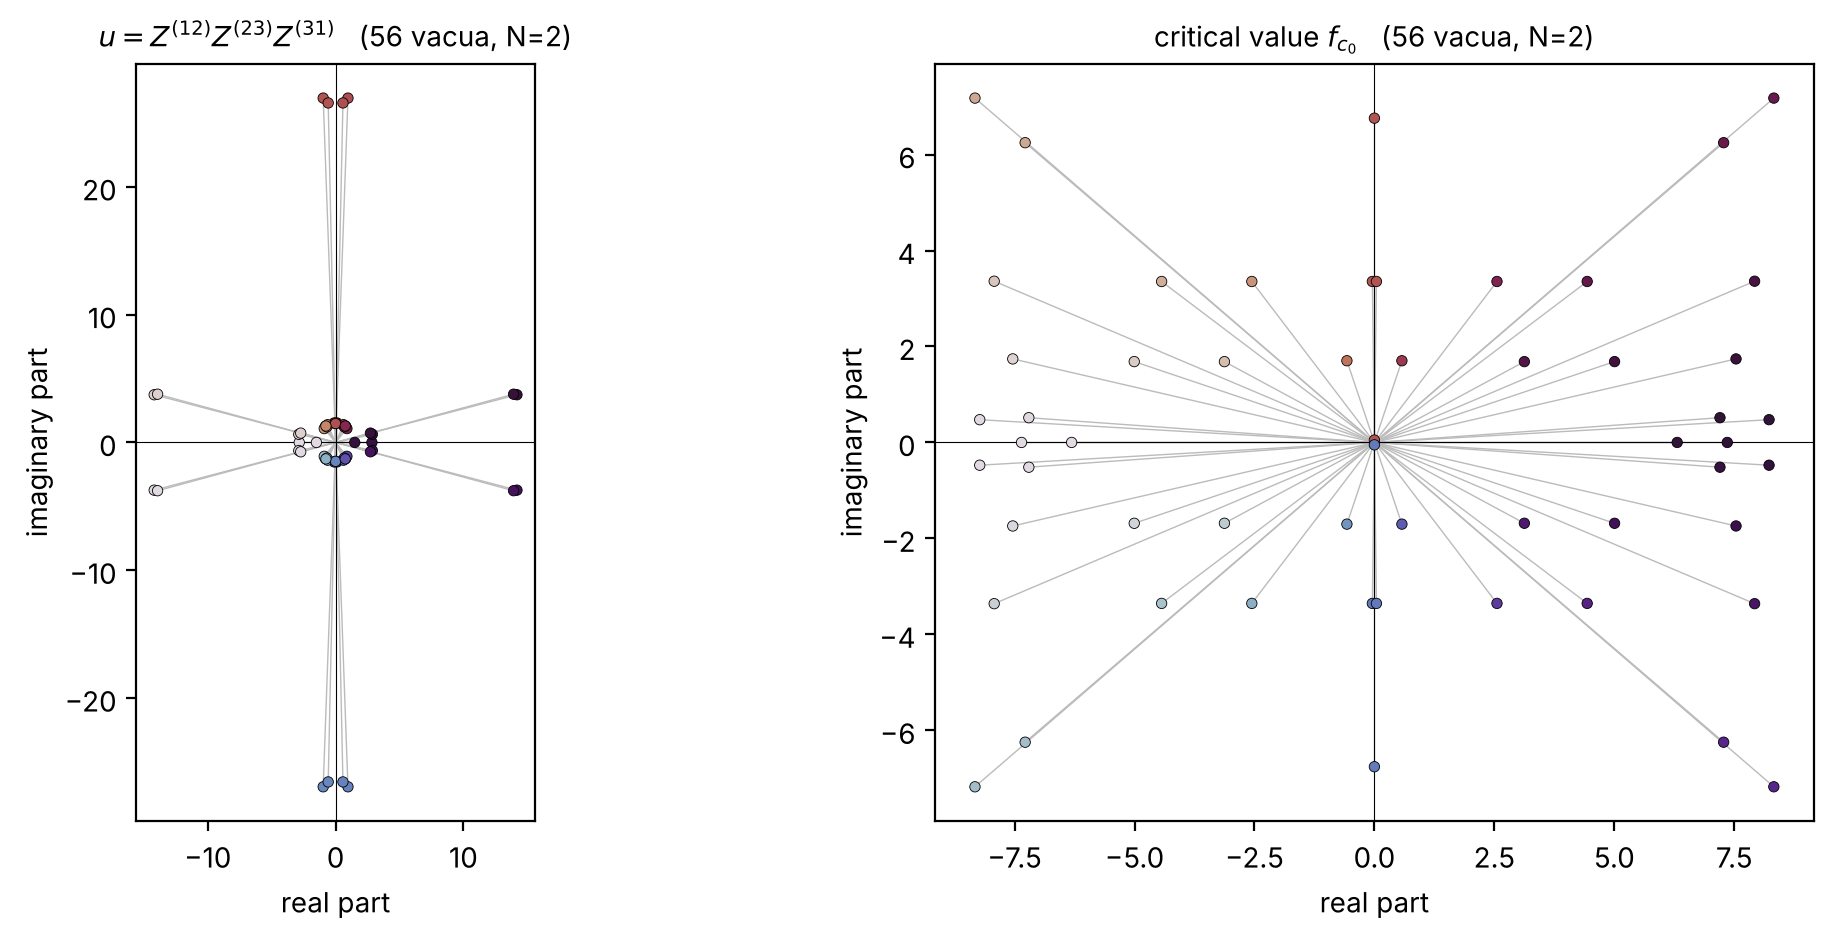
\includegraphics[width=0.98\textwidth]{figures/fig_N2.png}
\caption{The $56$ vacua of the $N=2$ system at $c=c_0$. Left: the gauge-invariant coordinate $u=Z^{(12)}Z^{(23)}Z^{(31)}$. Right: the critical values $f_{c_0}$. Points joined through the origin are exchanged by the involution $\sigma$ of Theorem~\ref{thm:A}(iv), which maps $u\mapsto-u$ and $f\mapsto-f$. Because $c_0$ is real, complex conjugation is a second symmetry, so the points also come in conjugate pairs.}
\label{fig:N2}
\end{figure}

\begin{figure}[t]
\centering
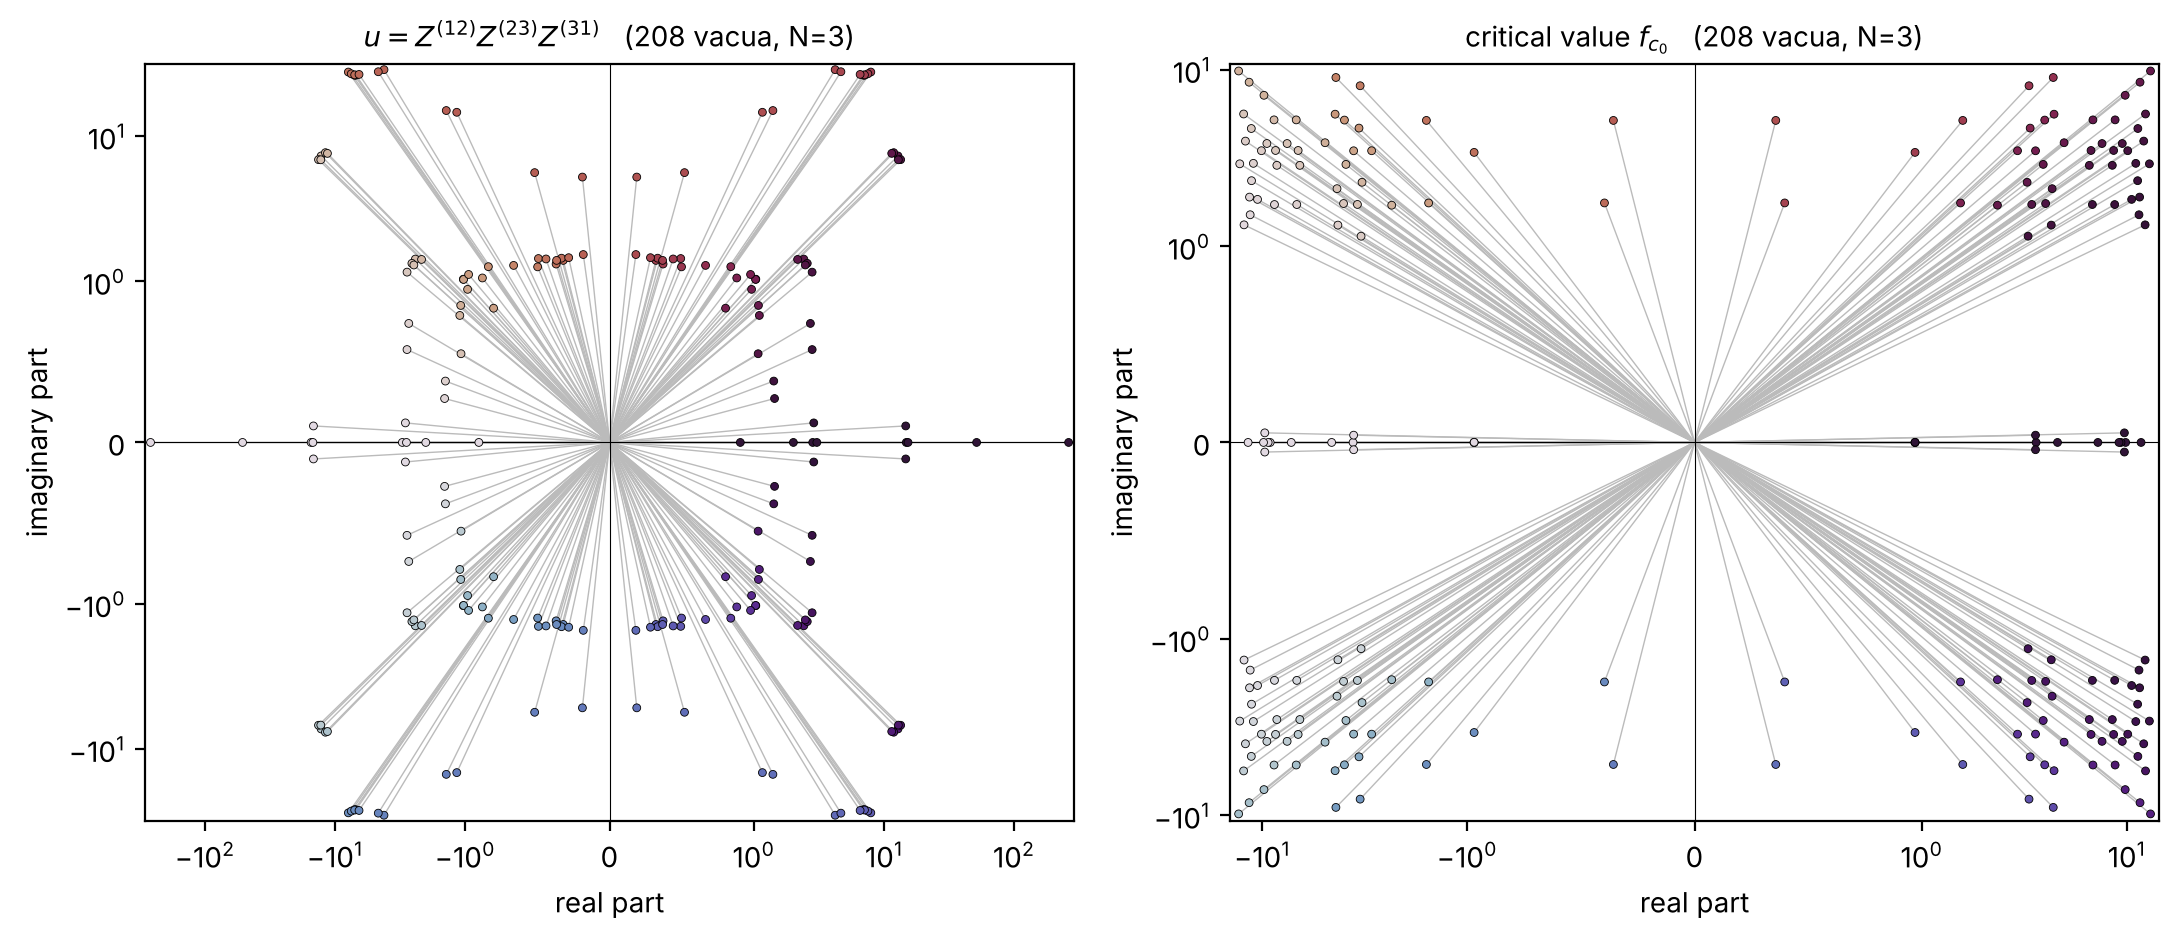
\includegraphics[width=0.98\textwidth]{figures/fig_N3.png}
\caption{The $208$ vacua of the $N=3$ system at $c=c_0$, drawn as in Figure~\ref{fig:N2} (both axes on a scale that is linear near $0$ and logarithmic beyond $1$). All $104$ pairs $\{p,\sigma p\}$ are visible as segments through the origin, and the $208$ critical values are distinct.}
\label{fig:N3}
\end{figure}

\section{Discussion}\label{sec:discussion}

\subsection{What is proved and what is not}
Theorem~\ref{thm:A} holds for every $N$ and every choice of parameters with $c^{(k\ell)}\ne0$. It reduces the conjecture to the statement that the regular function $f_c$ on the smooth variety $\cR^{\rm s}/\PG$ of dimension $2N^2+6N+13$ has exactly $-\hat c(4N)$ critical points modulo the $6$-dimensional group of shifts, for generic $c$, and it shows that the count is even whenever it is finite.

Theorem~\ref{thm:B} gives the count for $N=1$ at generic parameters and for $N=2,3$ at the explicit parameters $c_0$, together with a lower bound at generic parameters. The upper bound at generic parameters for $N=2,3$ is not proved. The reason is that we cannot show that $\Crit(f_c)$ is proper over the parameter space, that is, that no critical point escapes to infinity as $c$ approaches $c_0$. The usual argument would rescale $x=t\,y$ with $t\to\infty$: an escaping family of critical points of $\cW_c$ would approach a nonzero critical point of the cubic part of $\cW$, and one would like to show that there is none. But the cubic part does have nonzero critical points, for instance $Z^{(k\ell)}=0$ for all $k,\ell$ with commuting $\Phi^{(4)}_1,\Phi^{(4)}_2,\Phi^{(4)}_3$, so this argument does not apply. A proof of the generic upper bound would need either a Gröbner basis over the field of rational functions in the parameters, which is out of reach of present software for $N\ge2$, or a compactness argument that excludes vacua coming in from infinity.

\subsection{Larger \texorpdfstring{$N$}{N}}
The slice equations grow quickly with $N$: the slice has $3N^2+6N+15-(N^2+8)=2N^2+6N+7$ variables, so $27$, $43$, $63$ for $N=2,3,4$. The predicted number of solutions grows like $e^{2\pi\sqrt N}$ up to a power of $N$, the exponential of the entropy $\pi\sqrt{4N}$ of the corresponding black hole (Figure~\ref{fig:counts}).

\begin{figure}[t]
\centering
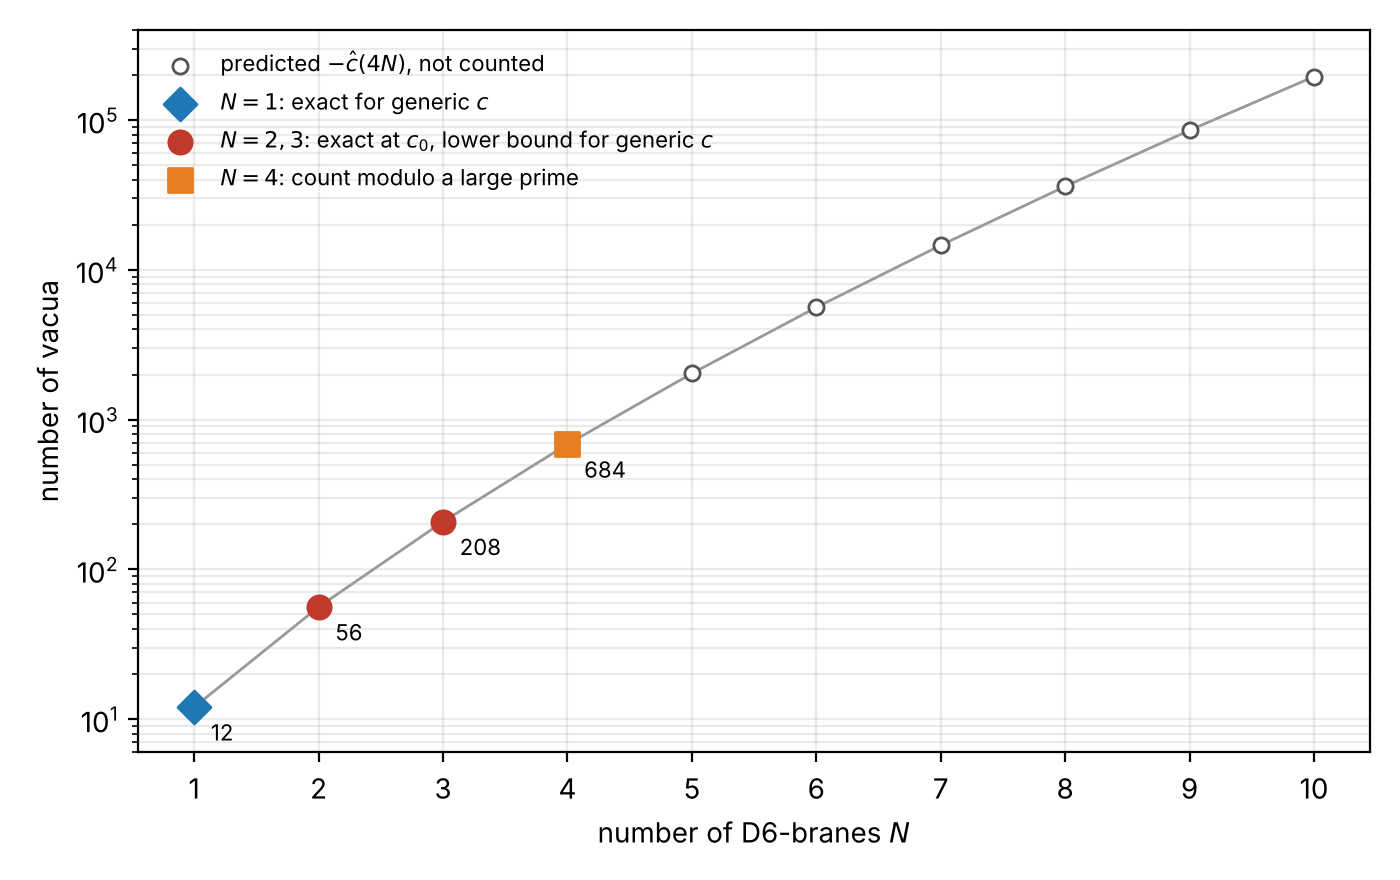
\includegraphics[width=0.8\textwidth]{figures/fig_counts.png}
\caption{The predicted number $-\hat c(4N)$ of vacua and the counts of this paper. For $N=4$ the count is modulo a prime and is not a proof.}
\label{fig:counts}
\end{figure}

\subsection{Other compactifications}
The same question can be asked for type~II string theory on $K3\times T^2$ and on Calabi--Yau threefolds, whose geometry includes fibrations by polarised $K3$ surfaces and quotients of $K3$ surfaces by involutions \cite{Bha22,BN26}. There multi-centred configurations contribute to the index, so a test of the strong conjecture must first separate the single-centred part, and a count of vacua alone does not suffice. The proof of Proposition~\ref{prop:simple} uses only two features of the equations: the bifundamentals between the $U(1)$ nodes are nonzero, and on the $U(N)$ node a commutator of adjoints equals a nonzero multiple of the identity up to a term whose image lies in the span of the incoming arrows and whose kernel contains the common kernel of the outgoing ones. Any quiver theory with these two features has only simple vacua.

\subsection{Two remarks on the structure}
First, the pairing of Theorem~\ref{thm:A}(iv) comes from the oddness of the superpotential, $\cW(-x)=-\cW(x)$, which holds because every term of $\cW$ has odd degree in the fields. It forces every count of isolated vacua to be even, for every $N$ and every $c$, in agreement with Lemma~\ref{lem:parity}, which shows that every $\hat c(4N)$ is even. Second, Proposition~\ref{prop:simple} does not involve the cubic couplings $\cW_2$ of the bifundamentals (Remark~\ref{rem:onetrace}), whereas the counts do: the authors of \cite{CGMS16} observe that for $N\ge2$ the result depends on the coefficient of $\cW_2$, which they fix by a string amplitude. All our computations use the superpotential \eqref{eq:W1}--\eqref{eq:W4} of \cite{CGMS16}.

\appendix

\section{The \texorpdfstring{$F$}{F}-term equations}\label{app:fterms}
With the convention of Lemma~\ref{lem:F}, the equations $\partial\cW/\partial\varphi=0$ are the following. For the adjoints they are \eqref{eq:F1}--\eqref{eq:F3}. For the bifundamentals between the $U(1)$ nodes:
\begin{align*}
(\Phi^{(1)}_3-\Phi^{(2)}_3)Z^{(21)}+Z^{(23)}Z^{(31)}+Z^{(24)}Z^{(41)}&=0, &&(Z^{(12)})\\
(\Phi^{(1)}_3-\Phi^{(2)}_3)Z^{(12)}+Z^{(13)}Z^{(32)}+Z^{(14)}Z^{(42)}&=0, &&(Z^{(21)})\\
(\Phi^{(3)}_2-\Phi^{(1)}_2)Z^{(31)}+Z^{(32)}Z^{(21)}-Z^{(34)}Z^{(41)}&=0, &&(Z^{(13)})\\
(\Phi^{(3)}_2-\Phi^{(1)}_2)Z^{(13)}+Z^{(12)}Z^{(23)}+Z^{(14)}Z^{(43)}&=0, &&(Z^{(31)})\\
(\Phi^{(2)}_1-\Phi^{(3)}_1)Z^{(32)}+Z^{(31)}Z^{(12)}+Z^{(34)}Z^{(42)}&=0, &&(Z^{(23)})\\
(\Phi^{(2)}_1-\Phi^{(3)}_1)Z^{(23)}+Z^{(21)}Z^{(13)}+Z^{(24)}Z^{(43)}&=0. &&(Z^{(32)})
\end{align*}
For the bifundamentals of the $U(N)$ node (columns of size $N$ first, then rows):
\begin{align}
(\Phi^{(1)}_1I_N-\Phi^{(4)}_1)Z^{(41)}+Z^{(42)}Z^{(21)}+Z^{(43)}Z^{(31)}&=0, &&(Z^{(14)})\notag\\
(\Phi^{(2)}_2I_N-\Phi^{(4)}_2)Z^{(42)}+Z^{(41)}Z^{(12)}+Z^{(43)}Z^{(32)}&=0, &&(Z^{(24)})\notag\\
(\Phi^{(3)}_3I_N-\Phi^{(4)}_3)Z^{(43)}-Z^{(41)}Z^{(13)}+Z^{(42)}Z^{(23)}&=0, &&(Z^{(34)})\notag\\
Z^{(14)}(\Phi^{(1)}_1I_N-\Phi^{(4)}_1)+Z^{(12)}Z^{(24)}-Z^{(13)}Z^{(34)}&=0, &&(Z^{(41)})\label{eq:Z41}\\
Z^{(24)}(\Phi^{(2)}_2I_N-\Phi^{(4)}_2)+Z^{(21)}Z^{(14)}+Z^{(23)}Z^{(34)}&=0, &&(Z^{(42)})\notag\\
Z^{(34)}(\Phi^{(3)}_3I_N-\Phi^{(4)}_3)+Z^{(31)}Z^{(14)}+Z^{(32)}Z^{(24)}&=0. &&(Z^{(43)})\notag
\end{align}
Each line is obtained by collecting the terms of $\cW$ that contain the given field and deleting that field, keeping the cyclic order: for instance $Z^{(12)}$ occurs in $\varepsilon^{123}\Phi^{(1)}_3Z^{(12)}Z^{(21)}$, $\varepsilon^{213}\Phi^{(2)}_3Z^{(21)}Z^{(12)}$, $Z^{(31)}Z^{(12)}Z^{(23)}$ and $\Tr(Z^{(12)}Z^{(24)}Z^{(41)})$. In total there are $6+6N+9+3N^2$ scalar equations, one for each coordinate of $\cR$. The list was checked against a symbolic differentiation of \eqref{eq:W1}--\eqref{eq:W4} for $N=1,2,3,4$ \cite{Bha26}.

\section{The predicted number of vacua}\label{app:prediction}
The Jacobi theta function is $\vartheta_1(z|\tau)=-iq^{1/8}(y^{1/2}-y^{-1/2})\prod_{n\ge1}(1-q^n)(1-q^ny)(1-q^n/y)$ with $q=e^{2\pi i\tau}$, $y=e^{2\pi iz}$, and $\eta(\tau)=q^{1/24}\prod_{n\ge1}(1-q^n)$, whose $24$th power is Ramanujan's cusp form $\Delta(\tau)=\sum_n\tau(n)q^n$ (see \cite{BBS23} for the function $\tau(n)$ and $PSL(2,\ZZ)$). Hence
\[
-\frac{\vartheta_1(z|\tau)^2}{\eta(\tau)^6}=(y-2+y^{-1})\prod_{n\ge1}\frac{(1-q^ny)^2(1-q^n/y)^2}{(1-q^n)^4}=\sum_{k\ge0,\ \ell\in\ZZ}\hat c(4k-\ell^2)\,q^ky^\ell .
\]
The coefficient depends only on $4k-\ell^2$, because $-\vartheta_1^2/\eta^6$ is a weak Jacobi form of weight $-2$ and index $1$ \cite{EZ85,SSY06}.\footnote{For a Jacobi form of index $1$ the coefficient of $q^ky^\ell$ is unchanged under $\ell\mapsto\ell+2$, $k\mapsto k+\ell+1$, which preserves $4k-\ell^2$, and under $\ell\mapsto-\ell$; both follow from the transformation laws of a Jacobi form \cite[Chapter~I]{EZ85}.} Expanding the product to order $q^{10}$ gives, for $N=0,1,\dots,10$,
\[
-\hat c(4N)=2,\,12,\,56,\,208,\,684,\,2032,\,5616,\,14592,\,36088,\,85500,\,195312 .
\]
The value $-\hat c(0)=2$ is the coefficient $-(-2)$ of $y^0$ in $y-2+y^{-1}$.

\begin{lemma}\label{lem:parity}
$\hat c(4N)$ is even for every $N\ge0$.
\end{lemma}

\begin{proof}
Work with power series in $q$ whose coefficients are Laurent polynomials in $y$ over $\ZZ/2$. There $(1-q^ny)^2=1-q^{2n}y^2$, $(1-q^n/y)^2=1-q^{2n}y^{-2}$, $(1-q^n)^4=1-q^{4n}$ and $y-2+y^{-1}=y+y^{-1}$. Hence modulo $2$ the series $-\vartheta_1^2/\eta^6$ equals $(y+y^{-1})F$, where $F$ involves only even powers of $y$. Every term of $(y+y^{-1})F$ has an odd power of $y$, so the coefficient of $q^Ny^0$ is even.
\end{proof}

Lemma~\ref{lem:parity} and Theorem~\ref{thm:A}(iv) are two independent explanations of the same parity, one on each side of the duality. For the D2-D2-D2-D6 system with $N$ D6-branes the index is $-\hat c(4N)$ \cite[Section~2]{CGMS16}, \cite{SSY06}.

\section{Certificates and data}\label{app:cert}
The archived programs \cite{Bha26} do the following.
\begin{enumerate}
\item Build $\cW$ symbolically, differentiate it, and impose the slice of Definition~\ref{def:slices} or an exceptional chart, at $c_0$ of Table~\ref{tab:c0}.
\item Eliminate linearly occurring variables and clear denominators.
\item Compute $\dim_\QQ\QQ[x]/I$ and the reduced Gröbner bases of the exceptional charts with the standard basis algorithm of Singular over $\QQ$, in exact arithmetic (not with modular methods, whose final test in Singular checks only that the input lies in the ideal of the result).
\item Compute rational univariate representations with msolve over $\QQ$.
\item Check each representation independently: parse $\chi$ and the $\rho_i$, verify that $\gcd(\chi,\chi')=1$, and reduce every equation at $x_i=\rho_i(t)$ modulo $\chi$ with exact rational arithmetic in FLINT.
\item For $N=4$, do the same modulo $p=2^{30}+3$ with arithmetic in $\mathbb F_p[t]$; this part is not a proof.
\end{enumerate}
The certificate files are part of the archive. Floating point numbers appear only in the figures, which locate the roots of $\chi$ with certified complex root isolation and evaluate the coordinates.

\section*{Declarations}

\noindent\textbf{Data availability.} The programs and the certificate files are archived at \cite{Bha26}.

\smallskip\noindent\textbf{Funding.} None.

\smallskip\noindent\textbf{Conflicts of interest.} None.

\begin{thebibliography}{99}

\bibitem{BBdBES12} I.~Bena, M.~Berkooz, J.~de~Boer, S.~El-Showk, D.~Van~den~Bleeken, \emph{Scaling BPS solutions and pure-Higgs states}, J. High Energy Phys. \textbf{2012}, no.~11 (2012), 171. doi:10.1007/JHEP11(2012)171

\bibitem{BBS23} D.~Bhattacharjee, P.~Bose, P.~Samal, \emph{Ramanujan $\tau$-function and its relationship with $PSL(2,\mathbb Z)$ for $\mathcal L_{24}(\tau)^{+,E}$}, Research Square (2023). doi:10.21203/rs.3.rs-2796280/v1

\bibitem{BES21} J.~Berthomieu, C.~Eder, M.~Safey El Din, \emph{msolve: a library for solving polynomial systems}, in: Proceedings of the 2021 International Symposium on Symbolic and Algebraic Computation (ISSAC '21), ACM, 2021, 51--58. doi:10.1145/3452143.3465545

\bibitem{Bha22} D.~Bhattacharjee, \emph{Generalization of quartic and quintic Calabi--Yau manifolds fibered by polarized K3 surfaces}, Research Square (2022). doi:10.21203/rs.3.rs-1965255/v1

\bibitem{Bha26} D.~Bhattacharjee, \emph{Code and certificates for: Black hole microstates of two and three D6-branes carry no angular momentum}, Zenodo (2026). doi:\zenodoDOI

\bibitem{BN26} D.~Bhattacharjee, P.~Nandi, \emph{Enriques and Kummer surfaces arising from K3 involutions}, Preprints (2026). doi:10.20944/preprints202602.0098.v1

\bibitem{CB01} W.~Crawley-Boevey, \emph{Geometry of the moment map for representations of quivers}, Compos. Math. \textbf{126} (2001), 257--293. doi:10.1023/A:1017558904030

\bibitem{CGMS14} A.~Chowdhury, R.~S.~Garavuso, S.~Mondal, A.~Sen, \emph{BPS state counting in $\mathcal N=8$ supersymmetric string theory for pure D-brane configurations}, J. High Energy Phys. \textbf{2014}, no.~10 (2014), 186. doi:10.1007/JHEP10(2014)186

\bibitem{CGMS16} A.~Chowdhury, R.~S.~Garavuso, S.~Mondal, A.~Sen, \emph{Do all BPS black hole microstates carry zero angular momentum?}, J. High Energy Phys. \textbf{2016}, no.~4 (2016), 082. doi:10.1007/JHEP04(2016)082

\bibitem{CLO15} D.~A.~Cox, J.~Little, D.~O'Shea, \emph{Ideals, Varieties, and Algorithms}, 4th ed., Undergraduate Texts in Mathematics, Springer, Cham, 2015. doi:10.1007/978-3-319-16721-3

\bibitem{DGMS11} A.~Dabholkar, J.~Gomes, S.~Murthy, A.~Sen, \emph{Supersymmetric index from black hole entropy}, J. High Energy Phys. \textbf{2011}, no.~4 (2011), 034. doi:10.1007/JHEP04(2011)034

\bibitem{Den02} F.~Denef, \emph{Quantum quivers and Hall/hole halos}, J. High Energy Phys. \textbf{2002}, no.~10 (2002), 023. doi:10.1088/1126-6708/2002/10/023

\bibitem{EZ85} M.~Eichler, D.~Zagier, \emph{The Theory of Jacobi Forms}, Progress in Mathematics \textbf{55}, Birkh\"auser, Boston, 1985. doi:10.1007/978-1-4684-9162-3

\bibitem{GP08} G.-M.~Greuel, G.~Pfister, \emph{A Singular Introduction to Commutative Algebra}, 2nd ed., Springer, Berlin, 2008. doi:10.1007/978-3-540-73542-7

\bibitem{Kin94} A.~D.~King, \emph{Moduli of representations of finite dimensional algebras}, Q. J. Math. \textbf{45} (1994), 515--530. doi:10.1093/qmath/45.4.515

\bibitem{MFK94} D.~Mumford, J.~Fogarty, F.~Kirwan, \emph{Geometric Invariant Theory}, 3rd ed., Ergebnisse der Mathematik und ihrer Grenzgebiete (2) \textbf{34}, Springer, Berlin, 1994. doi:10.1007/978-3-642-57916-5

\bibitem{Rou99} F.~Rouillier, \emph{Solving zero-dimensional systems through the rational univariate representation}, Appl. Algebra Engrg. Comm. Comput. \textbf{9} (1999), 433--461. doi:10.1007/s002000050114

\bibitem{Sen08b} A.~Sen, \emph{$\mathcal N=8$ dyon partition function and walls of marginal stability}, J. High Energy Phys. \textbf{2008}, no.~7 (2008), 118. doi:10.1088/1126-6708/2008/07/118

\bibitem{Sen10} A.~Sen, \emph{Arithmetic of $\mathcal N=8$ black holes}, J. High Energy Phys. \textbf{2010}, no.~2 (2010), 090. doi:10.1007/JHEP02(2010)090

\bibitem{Sen11} A.~Sen, \emph{How do black holes predict the sign of the Fourier coefficients of Siegel modular forms?}, Gen. Relativ. Gravit. \textbf{43} (2011), 2171--2183. doi:10.1007/s10714-011-1175-9

\bibitem{SSY06} D.~Shih, A.~Strominger, X.~Yin, \emph{Counting dyons in $\mathcal N=8$ string theory}, J. High Energy Phys. \textbf{2006}, no.~6 (2006), 037. doi:10.1088/1126-6708/2006/06/037

\bibitem{Wit82} E.~Witten, \emph{Constraints on supersymmetry breaking}, Nucl. Phys. B \textbf{202} (1982), 253--316. doi:10.1016/0550-3213(82)90071-2

\end{thebibliography}

\end{document}
